\documentclass[../main.tex]{subfiles}
\begin{document}

\theoremstyle{definition}

\chapter{Matrix Inverse and Condition}

\begin{center}
\textbf{CHAPTER OBJECTIVES}'
\end{center}
The primary objective of this chapter is to show how to compute the matrix inverse
and to illustrate how it can be used to analyze complex linear systems that occur in
engineering and science. In addition, a method to assess a matrix solution's sensitivity
to roundoff error is described. Specific objectives and topics covered are
\begin{itemize}
	\item Knowing how to determine the matrix inverse in an efficient manner based on LU
factorization.
	\item Understanding how the matrix inverse can be used to assess stimulus-response
characteristics of engineering systems.
	\item Understanding the meaning of matrix and vector norms and how they are computed.
	\item Knowing how to use norms to compute the matrix condition number.
	\item Understanding how the magnitude of the condition number can be used to
estimate the precision of solutions of linear algebraic equations.
\end{itemize}



\section{THE MATRIX INVERSE}

In our discussion of matrix operations (Section 8.1.2), we introduced the notion that if a matrix [A] is square, there is another matrix $[A]^{-1}$, called the inverse of [A], for which
\begin{equation}
[A][A]^{-1}=[A]^{-1}[A]=1
\tag{11.1}
\end{equation}
Now we will focus on how the inverse can be computed numerically. Then we will explore how it can be used for engineering analysis.

\subsection{Calculating the Inverse}
The inverse can be computed in a column-by-column fashion by generating solutions with unit vectors as the right-hand-side constants. For example, if the right-hand-side constant has a 1 in the first position and zeros elsewhere,

\begin{equation}
\{b\}=
\begin{Bmatrix}
1\\ 
0\\ 
0
\end{Bmatrix}
\tag{11.2}
\end{equation}

the resulting solution will be the first column of the matrix inverse. Similarly, if a unit vector with a 1 at the second row is used

\begin{equation}
\{b\}=
\begin{Bmatrix}
0\\ 
1\\ 
0
\end{Bmatrix}
\tag{11.3}
\end{equation}

the result will be the second column of the matrix inverse.
The best way to implement such a calculation is with LU factorization. Recall that one
of the great strengths of LU factorization is that it provides a very efficient means to evaluate multiple right-hand-side vectors.
Thus, it is ideal for evaluating the multiple unit vectors needed to compute the inverse.

\section*{EXAMPLE 11.1 Matrix Inversion}

Problem Statement. Employ LU factorization to determine the matrix inverse for the system from Example 10.1:

\begin{equation}
[A]=
\begin{bmatrix}
3 & -0.1 & -0.2 \\
0.1 & 7 & -0.2 \\
0.3 & -0.2 & 10
\end{bmatrix}
\end{equation}

Recall that the factorization resulted in the following lower and upper triangular matrices:

\begin{equation}
[U]=
\begin{bmatrix}
3 & -0.1 & -0.2 \\
0 & 7.00333 & -0.293333 \\
0 & 0 & 10.0120
\end{bmatrix}
\end{equation}

\begin{equation}
[L]=
\begin{bmatrix}
1 & 0 & 0 \\
0.0333333 & 1 & 0 \\
0.100000 & -0.0271300 & 1
\end{bmatrix}
\end{equation}

Solution. The first column of the matrix inverse can be determined by performing the forward-substitution solution procedure with a unit vector (with 1 in the first row) as the right-hand-side vector. Thus, the lower triangular system can be set up as (recall Eq. [10.8])
\begin{equation}
\begin{bmatrix}
1 & 0 & 0\\ 
0.0333333 & 1 & 0\\ 
0.100000 & -0.0271300 & 1
\end{bmatrix}
\begin{Bmatrix}
d_{1}\\ 
d_{2}\\ 
d_{3}
\end{Bmatrix}=\begin{Bmatrix}
1\\ 
0\\ 
0
\end{Bmatrix}
\end{equation}

and solved with forward substitution for $\{d\}6{T}=\left \lfloor 1 \;\;\; -0.03333 \;\;\; 0.1009 \right \rfloor$. This vector
can then be used as the right-hand side of the upper triangular system (recall Eq. [10.3]):

\begin{equation}
\begin{bmatrix}
3 & -0.1 & -0.2\\ 
0 & 7.00333 & -0.293333\\ 
0 & 0 &  10.0120
\end{bmatrix}
\begin{Bmatrix}
x_{1}\\ 
x_{2}\\ 
x_{3}
\end{Bmatrix}=\begin{Bmatrix}
1\\ 
-0.03333\\ 
-0.1009
\end{Bmatrix}
\end{equation}

which can be solved by back substitution for $\{x\}^{T}=\left \lfloor 0.33249 \; -0.00518 \; -0.01008 \right \rfloor$, which is the first column of the matrix inverse:

\begin{equation}
[A]^{-1}=\begin{bmatrix}
0.33249 & 0 &0 \\ 
-0.00518 & 0 & 0\\ 
-0.01008 & 0 & 0
\end{bmatrix}
\end{equation}

To determine the second column, Eq. (10.8) is formulated as
\begin{equation}
\begin{bmatrix}
1& 0& 0\\
0.0333333& 1& 0\\
0.100000& -0.0271300& 1
\end{bmatrix}
\begin{Bmatrix}
d_{1}\\ 
d_{2}\\ 
d_{3}
\end{Bmatrix}
=
\begin{Bmatrix}
0\\
1\\
0
\end{Bmatrix}
\end{equation}

This can be solved for $\{d\}$, and the results are used with Eq. (10.3) to determine 
$\{x\}^{T}=\left \lfloor 0.004944\;\;\; 0.142903\;\;\; 0.00271 \right \rfloor$
,which is the second column of the matrix inverse:
\begin{equation}
[A]^{-1}=
\begin{bmatrix}
0.33249& 0.004944& 0\\
-0.00518& 0.142903& 0\\
-0.01008& 0.002710& 0
\end{bmatrix}
\end{equation}

Finally, the same procedures can be implemented with $\{b\}^{T}=\left \lfloor 0\;\;\; 0\;\;\; 1 \right \rfloor$ to solve for
$\{x\}^{T}=\left \lfloor 0.006798\;\;\; 0.004183\;\;\; 0.09988 \right \rfloor$, which is the final column of the matrix inverse:
\begin{equation}
[A]^{-1}=
\begin{bmatrix}
0.33249& 0.004944& 0.006798\\
-0.00518& 0.142903& 0.004183\\
-0.01008& 0.002710& 0.099880
\end{bmatrix}
\end{equation}

The validity of this result can be checked by verifying that $[A][A]^{-1} = [I]$.

\subsection{Stimulus-Response Computations}
As discussed in PT 3.1, many of the linear systems of equations arising in engineering and science are derived from conservation laws. The mathematical expression of these laws
is some form of balance equation to ensure that a particular property—mass, force, heat,
momentum, electrostatic potential-is conserved. For a force balance on a structure, the
properties might be horizontal or vertical components of the forces acting on each node of the structure. For a mass balance, the properties might be the mass in each reactor of a chemical process. Other fields of engineering and science would yield similar examples.

A single balance equation can be written for each part of the system, resulting in a set
of equations defining the behavior of the property for the entire system. These equations
are interrelated, or coupled, in that each equation may include one or more of the variables from the other equations. For many cases, these systems are linear and, therefore, of the exact form dealt with in this chapter:
\begin{equation}
[A]\{x\}=\{b\}
\tag{11.4}
\end{equation}

Now, for balance equations, the terms of Eq. (11.4) have a definite physical interpretation. For example, the elements of $\{x\}$ are the levels of the property being balanced for each part of the system. In a force balance of a structure, they represent the horizontal and vertical forces in each member. For the mass balance, they are the mass of chemical in each reactor. In either case, they represent the system's state or response, which we are trying to determine.

The right-hand-side vector $\{b\}$ contains those elements of the balance that are independent of behavior of the system-that is, they are constants. In many problems, they
represent the forcing functions or external stimuli that drive the system.

Finally, the matrix of coefficients [A] usually contains the parameters that express
how the parts of the system interact or are coupled. Consequently, Eq. (11.4) might be
reexpressed as
\begin{equation}
[Interactions]\{response\}=\{stimuli\}
\end{equation}

As we know from previous chapters, there are a variety of ways to solve Eq. (11.4).
However, using the matrix inverse yields a particularly interesting result. The formal solution can be expressed as
\begin{equation}
\{x\} = [A]^{-1}\{b\}
\end{equation}
or (recalling our definition of matrix multiplication from Section 8.1.2)
\begin{equation}
x_{1} = a_{11}^{-1} b_{1} + a_{12}^{-1} b_{2} + a_{13}^{-1} b_{3}\\
x_{2} = a_{21}^{-1} b_{1} + a_{22}^{-1} b_{2} + a_{23}^{-1} b_{3}\\
x_{3} = a_{31}^{-1} b_{1} + a_{32}^{-1} b_{2} + a_{33}^{-1} b_{3}
\end{equation}
Thus, we find that the inverted matrix itself, aside from providing a solution, has extremely useful properties. That is, each of its elements represents the response of a single part of the system to a unit stimulus of any other part of the system.

Notice that these formulations are linear and, therefore, superposition and proportionality hold. Superposition means that if a system is subject to several different stimuli (the b's), the responses can be computed individually and the results summed to obtain a total response. Proportionality means that multiplying the stimuli by a quantity results in the response to those stimuli being multiplied by the same quantity. Thus, the coefficient $a_{11}^{-1}$ is a proportionality constant that gives the value of $x_{1}$ due to a unit level of $b_{1}$. This result is independent of the effects of $b_{2}$ and $b_{3}$ on $x_{1}$, which are reflected in the coefficients
$a_{12}^{-1}$ and $a_{13}^{-1}$ , respectively. Therefore, we can draw the general conclusion that the element $a_{ij}^{-1}$ of the inverted matrix represents the value of $x_{i}$ due to a unit quantity of $b_{j}$.

Using the example of the structure, element $a_{ij}^{-1}$ of the matrix inverse would represent the force in member i due to a unit external force at node j. Even for small systems, such behavior of individual stimulus-response interactions would not be intuitively obvious. As such, the matrix inverse provides a powerful technique for understanding the interrelationships of component parts of complicated systems.

\section*{EXAMPLE 11.2 Analyzing the Bungee Jumper Problem}

Problem Statement. At the beginning of Chap. 8, we set up a problem involving three
individuals suspended vertically connected by bungee cords. We derived a system of linear
algebraic equations based on force balances for each jumper,

\begin{equation}
\begin{bmatrix}
150& -100& 0\\
-100& 150& -50\\
0& -50& 50
\end{bmatrix}
\begin{Bmatrix}
x_{1}\\ 
x_{2}\\ 
x_{3}
\end{Bmatrix}
=
\begin{Bmatrix}
588.6\\
686.7\\
784.8
\end{Bmatrix}
\end{equation}

In Example 8.2, we used MATLAB to solve this system for the vertical positions of the
jumpers (the x's). In the present example, use MATLAB to compute the matrix inverse and
interpret what it means.

Solution. Start up MATLAB and enter the coefficient matrix:
\begin{lstlisting}[numbers=none]
>> K = [150 -100 0;-100 150 -50;0 -50 50];
\end{lstlisting}
The inverse can then be computed as 
\begin{lstlisting}[numbers=none]
>> KI = inv(K)
KI =
	0.0200 0.0200 0.0200
	0.0200 0.0300 0.0300
	0.0200 0.0300 0.0500
\end{lstlisting}

Each element of the inverse, $k_{ij}^{-1}$ of the inverted matrix represents the vertical change in position (in meters) of jumper i due to a unit change in force (in Newtons) applied to jumper j. 

First, observe that the numbers in the first column ($j = 1$) indicate that the position of all three jumpers would increase by 0.02 m if the force on the first jumper was increased by 1 N. This makes sense, because the additional force would only elongate the first cord by that amount.

In contrast, the numbers in the second column ($j = 2$) indicate that applying a force
of 1 N to the second jumper would move the first jumper down by 0.02 m, but the second
and third by 0.03 m. The 0.02-m elongation of the first jumper makes sense because the
first cord is subject to an extra 1 N regardless of whether the force is applied to the first or second jumper. However, for the second jumper the elongation is now 0.03 m because along with the first cord, the second cord also elongates due to the additional force. And of course, the third jumper shows the identical translation as the second jumper as there is no additional force on the third cord that connects them.

As expected, the third column ($j = 3$) indicates that applying a force of 1 N to the
third jumper results in the first and second jumpers moving the same distances as occurred when the force was applied to the second jumper. However, now because of the additional elongation of the third cord, the third jumper is moved farther downward.

Superposition and proportionality can be demonstrated by using the inverse to determine how much farther the third jumper would move downward if additional forces of 10,
50, and 20 N were applied to the first, second, and third jumpers, respectively. This can be done simply by using the appropriate elements of the third row of the inverse to compute,
\begin{equation}
\Delta x_{3} = k_{31}^{-1} \Delta F_{1} +k_{32}^{-1} \Delta F_{2} +k_{33}^{-1} \Delta F_{3} = 0.02(10) + 0.03(50) + 0.05(20) = 2.7 m
\end{equation}

\section{ERROR ANALYSIS AND SYSTEM CONDITION}
Aside from its engineering and scientific applications, the inverse also provides a means to
discern whether systems are ill-conditioned. Three direct methods can be devised for this purpose:
\begin{enumerate}
\item Scale the matrix of coefficients $[A]$ so that the largest element in each row is 1. Invert the scaled matrix and if there are elements of $[A]^{-1}$ that are several orders of magnitude greater than one, it is likely that the system is ill-conditioned.
\item Multiply the inverse by the original coefficient matrix and assess whether the result is close to the identity matrix. If not, it indicates ill-conditioning.
\item Invert the inverted matrix and assess whether the result is sufficiently close to the original coefficient matrix. If not, it again indicates that the system is ill-conditioned.
\end{enumerate}
Although these methods can indicate ill-conditioning, it would be preferable to obtain
a single number that could serve as an indicator of the problem. Attempts to formulate such
a matrix condition number are based on the mathematical concept of the norm.

\subsection{Vector and Matrix Norms}

A norm is a real-valued function that provides a measure of the size or "length" of multicomponent mathematical entities such as vectors and matrices.

A simple example is a vector in three-dimensional Euclidean space (Fig. 11.1) that can be represented as
\begin{equation}
\left \lfloor F \right \rfloor =\left \lfloor a\;\;b\;\;c \right \rfloor 
\end{equation}
where a, b, and c are the distances along the x, y, and z axes, respectively. The length of this vector-that is, the distance from the coordinate (0, 0, 0) to (a, b, c)-can be simply computed as
\begin{equation}
\left \| F \right \|_{e}=
\sqrt{a^{2}+b^{2}+c^{2}}
\end{equation}

where the nomenclature $\left \| F \right \|_{e}$ indicates that this length is referred to as the Euclidean norm of [F].

Similarly, for an n-dimensional vector $\left \lfloor X \right \rfloor = \left \lfloor x_{1}\;\; x_{2}\;\; \cdots \;\; x_{n} \right \rfloor$, a Euclidean norm would be computed as

\begin{equation}
\left \| X \right \|_{e}=
\sqrt{\sum_{i=1}^{n}x_{i}^{2}}
\end{equation}
\begin{figure}[H]
	\centering
	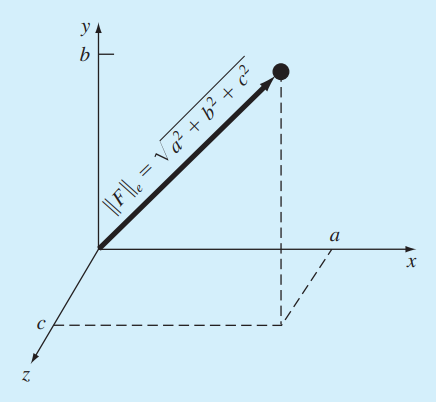
\includegraphics[width=0.75\textwidth]{fig_11_16}
	\caption{\textsf{Graphical depiction of a vector in Euclidean space.}}
	\label{fig:fig_11_16}
\end{figure}

The concept can be extended further to a matrix [A], as in

\begin{equation}
\left \| A \right \|_{f}=
\sqrt{\sum_{i=1}^{n}\sum_{j=1}^{n}a_{i,j}^{2}}
\tag{11.5}
\end{equation}
which is given a special name-the Frobenius norm. As with the other vector norms, it provides a single value to quantify the "size" of [A].

It should be noted that there are alternatives to the Euclidean and Frobenius norms. For vectors, there are alternatives called p norms that can be represented generally by
\begin{equation}
\left \| X \right \|_{p}=
\left ( \sum_{i=1}^{n}\left | x_{i} \right |^{p} \right )^{1/p}
\end{equation}

We can see that the Euclidean norm and the 2 norm,$\left \| X \right \|_{2}$, are identical for vectors. Other important examples are (p = 1)
\begin{equation}
\left \| X \right \|_{1}=
\left ( \sum_{i=1}^{n}\left | x_{i} \right | \right )
\end{equation}

which represents the norm as the sum of the absolute values of the elements. Another is the maximum-magnitude or uniform-vector norm (p = $\infty$),
\begin{equation}
\left \| X \right \|_{\infty}=
\underset{1\leq j\leq n}{max}\left | x_{i} \right |
\end{equation}
which defines the norm as the element with the largest absolute value

Using a similar approach, norms can be developed for matrices. For example,
\begin{equation}
\left \| A \right \|_{1}=
\underset{1\leq j\leq n}{max}\sum_{i=1}^{n}\left | a_{ij} \right |
\end{equation}
That is, a summation of the absolute values of the coefficients is performed for each column, and the largest of these summations is taken as the norm. This is called the columnsum norm.

A similar determination can be made for the rows, resulting in a uniform-matrix or row-sum norm:
\begin{equation}
\left \| A \right \|_{\infty}=
\underset{1\leq j\leq n}{max}\sum_{i=1}^{n}\left | a_{ij} \right |
\end{equation}

It should be noted that, in contrast to vectors, the 2 norm and the Frobenius norm for a matrix are not the same. Whereas the Frobenius norm $\left \| A \right \|_{f}$ can be easily determined by Eq. (11.5), the matrix 2 norm $\left \| A \right \|_{2}$ is calculated as
\begin{equation}
\left \| A \right \|_{2}=(\mu_{max})^{1/2}
\end{equation}

where $\mu_{max}$ is the largest eigenvalue of $[A]^{T} [A]$. In Chap. 13, we will learn more about eigenvalues. For the time being, the important point is that the $\left \| A \right \|_{2}$, or spectral norm, is the minimum norm and, therefore, provides the tightest measure of size (Ortega, 1972).

\subsection{Matrix Condition Number}
Now that we have introduced the concept of the norm, we can use it to define
$$Cond[A] = \left \| A \right \| \cdot \left \| A^{-1} \right \|$$

where Cond[A] is called the matrix condition number. Note that for a matrix [A], this number will be greater than or equal to 1. It can be shown (Ralston and Rabinowitz, 1978; Gerald and Wheatley, 1989) that

$$ \frac{\left \| \Delta X \right \|}{\left \| X \right \|}\leq Cond[A]\tfrac{\left \| \Delta A \right \|}{\left \| A \right \|}$$

That is, the relative error of the norm of the computed solution can be as large as the relative error of the norm of the coefficients of [A] multiplied by the condition number. For example, if the coefficients of [A] are known to t-digit precision (i.e., rounding errors are on
the order of $10^{-t}$) and $Cond[A] - 10^{c}$ , the solution [X] may be valid to only $t - c$ digits (rounding errors $\thickapprox 10^{c-t}$ ).

\section*{EXAMPLE 11.3 Matrix Condition Evaluation}

Problem Statement. The Hilbert matrix, which is notoriously ill-conditioned, can be represented generally as
\begin{equation}
\begin{bmatrix}
1 &\frac{1}{2}  &\frac{1}{3}  & \cdots  &\frac{1}{n} \\ 
\frac{1}{2}  &\frac{1}{3}  &\frac{1}{4}  &\cdots  &\frac{1}{n+1} \\ 
\vdots &\vdots  &\vdots  &  &\vdots \\ 
\frac{1}{n} &\frac{1}{n+1}  &\frac{1}{n+2}  &\cdots   &\frac{1}{2n+1}
\end{bmatrix}
\end{equation}

Use the row-sum norm to estimate the matrix condition number for the $3\times3$ Hilbert matrix:
\begin{equation}
[A]=
\begin{bmatrix}
1 &\frac{1}{2}  &\frac{1}{3} \\
\frac{1}{2} &\frac{1}{3}  &\frac{1}{4} \\
\frac{1}{3} &\frac{1}{4}  &\frac{1}{5}
\end{bmatrix}
\end{equation}

Solution. First, the matrix can be normalized so that the maximum element in each row is 1:

\begin{equation}
[A]=
\begin{bmatrix}
1 &\frac{1}{2}  &\frac{1}{3} \\
1 &\frac{2}{3}  &\frac{1}{2} \\
1 &\frac{3}{4}  &\frac{3}{5}
\end{bmatrix}
\end{equation}

Summing each of the rows gives 1.833, 2.1667, and 2.35. Thus, the third row has the largest sum and the row-sum norm is
\begin{equation}
\left \| A \right \|_{\infty}=1+\frac{3}{4}+\frac{3}{5}=2.35
\end{equation}

The inverse of the scaled matrix can be computed as
\begin{equation}
[A]^{-1}=
\begin{bmatrix}
9& -18& 10\\
-36& 96& -60\\
30& -90& 60
\end{bmatrix}
\end{equation}

Note that the elements of this matrix are larger than the original matrix. This is also reflected in its row-sum norm, which is computed as
\begin{equation}
\left \| A^{-1} \right \|_{\infty}=\left | -36 \right |+
\left | 96 \right |+ \left | -60 \right |=192
\end{equation}

Thus, the condition number can be calculated as

$$Cond[A] = 2.35(192) = 451.2$$

The fact that the condition number is much greater than unity suggests that the system is ill-conditioned. The extent of the ill-conditioning can be quantified by calculating
$c = log 451.2 = 2.65$. Hence, the last three significant digits of the solution could exhibit
rounding errors. Note that such estimates almost always overpredict the actual error. However,
they are useful in alerting you to the possibility that roundoff errors may be significant.

\subsection{Norms and Condition Number in MATLAB}

MATLAB has built-in functions to compute both norms and condition numbers:
\begin{lstlisting}[numbers=none]
>> norm(X,p)
\end{lstlisting}
and
\begin{lstlisting}[numbers=none]
>> cond(X,p)
\end{lstlisting}
where X is the vector or matrix and p designates the type of norm or condition number (1, 2, inf, or 'fro'). Note that the cond function is equivalent to
\begin{lstlisting}[numbers=none]
>> norm(X,p) * norm(inv(X),p)
\end{lstlisting}
Also, note that if p is omitted, it is automatically set to 2.

\section*{EXAMPLE 11.4 Matrix Condition Evaluation with MATLAB}

Problem Statement. Use MATLAB to evaluate both the norms and condition numbers
for the scaled Hilbert matrix previously analyzed in Example 11.3:

\begin{equation}
\begin{bmatrix}
1 &\frac{1}{2}  &\frac{1}{3} \\ 
1  &\frac{2}{3}  &\frac{1}{2} \\ 
1  &\frac{3}{4}  &\frac{3}{5}
\end{bmatrix}
\end{equation}

(a) As in Example 11.3, first compute the row-sum versions (p = inf). (b) Also compute the Frobenius (p = 'fro') and the spectral (p = 2) condition numbers.

Solution: (a) First, enter the matrix:

\begin{lstlisting}[numbers=none]
>> A = [1 1/2 1/3;1 2/3 1/2;1 3/4 3/5];
\end{lstlisting}

Then, the row-sum norm and condition number can be computed as

\begin{lstlisting}[numbers=none]
>> norm(A,inf)
ans =
	2.3500
>> cond(A,inf)
ans =
	451.2000
\end{lstlisting}

These results correspond to those that were calculated by hand in Example 11.3. (b) The condition numbers based on the Frobenius and spectral norms are

\begin{lstlisting}[numbers=none]
>> cond(A,'fro')
ans =
	368.0866
>> cond(A)
ans =
	366.3503
\end{lstlisting}


\section{CASE STUDY INDOOR AIR POLLUTION}

Background. As the name implies, indoor air pollution deals with air contamination
in enclosed spaces such as homes, offices, and work areas. Suppose that you are studying
the ventilation system for Bubba's Gas 'N Guzzle, a truck-stop restaurant located adjacent
to an eight-lane freeway.

As depicted in Fig. 11.2, the restaurant serving area consists of two rooms for smokers
and kids and one elongated room. Room 1 and section 3 have sources of carbon monoxide
from smokers and a faulty grill, respectively. In addition, rooms 1 and 2 gain carbon
monoxide from air intakes that unfortunately are positioned alongside the freeway. 
\begin{figure}[H]
	\centering
	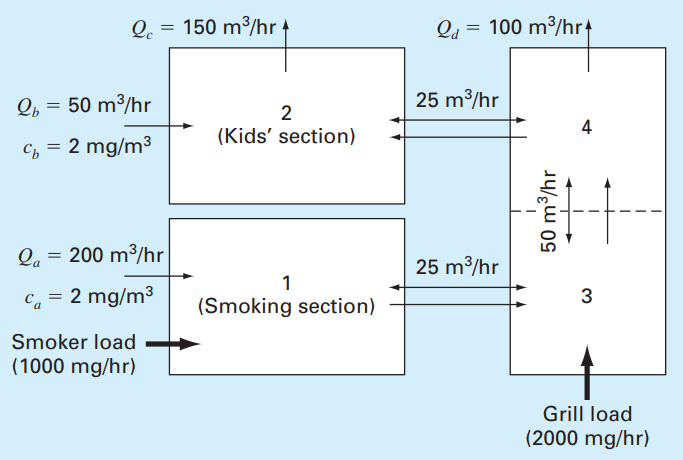
\includegraphics[width=0.75\textwidth]{fig_11_17}
	\caption{\textsf{Overhead view of rooms in a restaurant. The one-way arrows represent volumetric airflows,
whereas the two-way arrows represent diffusive mixing. The smoker and grill loads add carbon
monoxide mass to the system but negligible airflow}}
	\label{fig:fig_11_17}
\end{figure}

Write steady-state mass balances for each room and solve the resulting linear algebraic equations for the concentration of carbon monoxide in each room. In addition, generate the matrix inverse and use it to analyze how the various sources affect the kids'
room. For example, determine what percent of the carbon monoxide in the kids' section is
due to (1) the smokers, (2) the grill, and (3) the intake vents. In addition, compute the improvement in the kids' section concentration if the carbon monoxide load is decreased by
banning smoking and fixing the grill. Finally, analyze how the concentration in the kids'
area would change if a screen is constructed so that the mixing between areas 2 and 4 is
decreased to 5 $m^{3}/hr$.

Solution. Steady-state mass balances can be written for each room. For example, the balance for the smoking section (room 1) is
\begin{equation}
0 = W_{smoker} + Q_{a}c_{a} - Q_{a}c_{1} + E_{13}(c_{3} - c_{1})\\
(Load) + (In o w) - (Out o w) + (Mixing)
\end{equation}

Similar balances can be written for the other rooms:
\begin{equation}
0 = Q_{b}c_{b} + (Q_{a} - Q_{d})c_{4} - Q_{c}c_{2} + E_{24}(c_{4} - c_{2})\\
0 = W_{grill} + Q_{a}c_{1} + E_{13}(c_{1} - c_{3}) + E_{34}(c_{4} - c_{3}) - Q_{a}c_{3}\\
0 = Q_{a}c_{3} + E_{34}(c_{3} - c_{4}) + E_{24}(c_{2} - c_{4}) - Q_{a}c_{4}
\end{equation}

Substituting the parameters yields the final system of equation:
\begin{equation}
\begin{bmatrix}
225& 0& -25& 0\\
0& 175& 0& -125\\
-225& 0& 275& -50\\
0& -25& -250& 275
\end{bmatrix}
\begin{Bmatrix}
c_{1}\\ 
c_{2}\\ 
c_{3}\\ 
c_{4}
\end{Bmatrix}
=
\begin{Bmatrix}
1400\\
100\\
2000\\
0
\end{Bmatrix}
\end{equation}

MATLAB can be used to generate the solution. First, we can compute the inverse. Note that we use the "short g" format in order to obtain five significant digits of precision:

\begin{lstlisting}[numbers=none]
>> format short g
>> A=[225 0 -25 0
0 175 0 -125
-225 0 275 -50
0 -25 -250 275];
>> AI=inv(A)
AI =
	0.0049962 	1.5326e-005	0.00055172 	0.00010728
	0.0034483 	0.0062069 	0.0034483 	0.0034483
	0.0049655 	0.00013793 	0.0049655 	0.00096552
	0.0048276 	0.00068966 	0.0048276 	0.0048276
\end{lstlisting}

The solution can then be generated as
\begin{lstlisting}[numbers=none]
>> b=[1400 100 2000 0]';
>> c=AI*b
c =
	8.0996
	12.345
	16.897
	16.483
\end{lstlisting}
Thus, we get the surprising result that the smoking section has the lowest carbon
monoxide levels! The highest concentrations occur in rooms 3 and 4 with section 2 having
an intermediate level. These results take place because (a) carbon monoxide is conservative and (b) the only air exhausts are out of sections 2 and 4 ($Q_{c}$ and $Q_{d}$). Room 3 is so bad
because not only does it get the load from the faulty grill, but it also receives the effluent
from room 1.

Although the foregoing is interesting, the real power of linear systems comes from
using the elements of the matrix inverse to understand how the parts of the system interact.
For example, the elements of the matrix inverse can be used to determine the percent of the
carbon monoxide in the kids' section due to each source:

The smokers:
\begin{equation}
c_{2,smokers} = a_{21}^{-1} W_{smokers} = 0.0034483(1000) = 3.4483\\
\%_{smokers} = \frac{3.4483}{12.345} \times 100\% = 27.93\%
\end{equation}

The grill:
\begin{equation}
c_{2,grill} = a_{23}^{-1} W_{grill} = 0.0034483(2000) = 6.897\\
\%_{grill} = \frac{6.897}{12.345} \times 100\% = 55.87\%
\end{equation}

The intakes:
\begin{equation}
c_{2,intakes} = a_{21}^{-1} Q_{a}c_{a} + a_{22}^{-1} Q_{b}c_{b} = 0.0034483(200)2 + 0.0062069(50)2
= 1.37931 + 0.62069 = 2\\
\%_{grill} = \frac{2}{12.345}\times 100\% = 16.20\%
\end{equation}
The faulty grill is clearly the most significant source.

The inverse can also be employed to determine the impact of proposed remedies such
as banning smoking and fixing the grill. Because the model is linear, superposition holds
and the results can be determined individually and summed:
\begin{equation}
\vartriangle c_{2} = a_{21}^{-1} \vartriangle W_{smoker} + a_{23}^{-1} \vartriangle W_{grill} = 0.0034483(-1000) + 0.0034483(-2000)\\
= -3.4483 - 6.8966 = -10.345
\end{equation}

Note that the same computation would be made in MATLAB as
\begin{lstlisting}[numbers=none]
>> AI(2,1)*(-1000)+AI(2,3)*(-2000)
ans =
	-10.345
\end{lstlisting}

Implementing both remedies would reduce the concentration by $10.345 mg/m^{3}$. The result would bring the kids' room concentration to $12.345 - 10.345 = 2 mg/m^{3}$. This makes sense, because in the absence of the smoker and grill loads, the only sources are the air intakes which are at $2 mg/m^{3}$. 

Because all the foregoing calculations involved changing the forcing functions, it was
not necessary to recompute the solution. However, if the mixing between the kids' area and
zone 4 is decreased, the matrix is changed
\begin{equation}
\begin{bmatrix}
225& 0& -25& 0\\
0& 155& 0& -105\\
-225& 0& 275& -50\\
0& -5& -250& 255
\end{bmatrix}
\begin{Bmatrix}
c_{1}\\ 
c_{2}\\ 
c_{3}\\ 
c_{4}
\end{Bmatrix}
=
\begin{Bmatrix}
1400\\
100\\
2000\\
0
\end{Bmatrix}
\end{equation}

The results for this case involve a new solution. Using MATLAB, the result is
\begin{equation}
\begin{Bmatrix}
c_{1}\\ 
c_{2}\\ 
c_{3}\\ 
c_{4}
\end{Bmatrix}
=
\begin{Bmatrix}
8.1084\\
12.0800\\
16.9760\\
16.8800
\end{Bmatrix}
\end{equation}

Therefore, this remedy would only improve the kids' area concentration by a paltry $0.265 mg/m^{3}$. 


\section*{PROBLEMS}


11.1 Determine the matrix inverse for the following system:
\begin{equation}
10x_{1} + 2x_{2} - x_{3} = 27\\
-3x_{1} - 6x_{2} + 2x_{3} = -61.5\\
x_{1} + x_{2} + 5x_{3} = -21.5
\end{equation}
Check your results by verifying that $[A][A]^{-1} = [I]$. Do not use a pivoting strategy.


11.2 Determine the matrix inverse for the following system:
\begin{equation}
-8x_{1} + x_{2} - 2x_{3} = -20
2x_{1} - 6x_{2} - x_{3} = -38
-3x_{1} - x_{2} + 7x_{3} = -34
\end{equation}


11.3 The following system of equations is designed to
determine concentrations (the c's in $g/m^{3}$) in a series of
coupled reactors as a function of the amount of mass input to
each reactor (the right-hand sides in g/day):
\begin{equation}
15c_{1} - 3c_{2} - c_{3} = 4000
-3c_{1} + 18c_{2} - 6c_{3} = 1500
-4c_{1} - c_{2} + 12c_{3} = 2400
\end{equation}
(a) Determine the matrix inverse.

(b) Use the inverse to determine the solution.

(c) Determine how much the rate of mass input to reactor 3
must be increased to induce a 10 $g/m^{3}$ rise in the concentration of reactor 1.

(d) How much will the concentration in reactor 3 be reduced if the rate of mass input to reactors 1 and 2 isreduced by 500 and 250 g/day, respectively?


11.4 Determine the matrix inverse for the system described
in Prob. 8.9. Use the matrix inverse to determine the
concentration in reactor 5 if the inflow concentrations are
changed to $c_{01} = 10$ and $c_{03} = 20$.


11.5 Determine the matrix inverse for the system described
in Prob. 8.10. Use the matrix inverse to determine the force
in the three members ($F_{1}$, $F_{2}$ and $F_{3}$) if the vertical load at
node 1 is doubled to $F_{1,v} = -4000 N$ and a horizontal load
of $F_{3,h} = -1000 N$ is applied to node 3.


11.6 Determine $\left \|A_{f}\right \|$ , $\left \|A_{1}\right \|$, and $\left \|A\right \|_{\infty}$ for
\begin{equation}
[A]=
\begin{bmatrix}
8& 2& -10\\
-9&1& 3\\
15& -1& 6
\end{bmatrix}
\end{equation}
Before determining the norms, scale the matrix by making
the maximum element in each row equal to one.


11.7 Determine the Frobenius and row-sum norms for the
systems in Probs. 11.2 and 11.3.


11.8 Use MATLAB to determine the spectral condition number for the following system. Do not normalize the system:
\begin{equation}
\begin{bmatrix}
1& 4& 9& 16& 25\\
4& 9& 16& 25& 36\\
9& 16& 25& 36& 49\\
16& 25& 36& 49& 64\\
25& 36& 49& 64& 81
\end{bmatrix}
\end{equation}
Compute the condition number based on the row-sum norm.


11.9 Besides the Hilbert matrix, there are other matrices
that are inherently ill-conditioned. One such case is the
Vandermonde matrix, which has the following form:
\begin{equation}
\begin{bmatrix}
x_{1}^{2}& x_{1}& 1\\
x_{2}^{2}& x_{2}& 1\\
x_{3}^{2}& x_{3}& 1\\
\end{bmatrix}
\end{equation}

(a) Determine the condition number based on the row-sum
norm for the case where $x_{1} = 4$, $x_{2} = 2$, and $x_{3} = 7$.

(b) Use MATLAB to compute the spectral and Frobenius
condition numbers.


11.10 Use MATLAB to determine the spectral condition
number for a 10-dimensional Hilbert matrix. How many digits of precision are expected to be lost due to ill-conditioning?
Determine the solution for this system for the case where each
element of the right-hand-side vector $\{b\}$ consists of the summation of the coefficients in its row. In other words, solve for
the case where all the unknowns should be exactly one. Compare the resulting errors with those expected based on the
condition number.


11.11 Repeat Prob. 11.10, but for the case of a sixdimensional Vandermonde matrix (see Prob. 11.9) where
$x_{1} = 4$, $x_{2} = 2$, $x_{3} = 7$, $x_{4} = 10$, $x_{5} = 3$, and $x_{6} = 5$.


11.12 The Lower Colorado River consists of a series of four
reservoirs as shown in Fig. P11.12.

Mass balances can be written for each reservoir, and
the following set of simultaneous linear algebraic equations
results:
\begin{equation}
\begin{bmatrix}
13.422 &0 &0 &0 \\ 
-13.422 &12.252 &0 &0 \\ 
0 &-12.252 &12.377 &0 \\ 
0 &0 &-12.377 & 11.797
\end{bmatrix}
\times 
\begin{Bmatrix}
c_{1}\\ 
c_{2}\\ 
c_{3}\\ 
c_{4}
\end{Bmatrix}
=
\begin{Bmatrix}
750.5\\
300\\
102\\
30
\end{Bmatrix}
\end{equation}
where the right-hand-side vector consists of the loadings of
chloride to each of the four lakes and $c_{1}$, $c_{2}$, $c_{3}$, and $c_{4}$ = the resulting chloride concentrations for Lakes Powell, Mead,
Mohave, and Havasu, respectively.

(a) Use the matrix inverse to solve for the concentrations in
each of the four lakes.

(b) How much must the loading to Lake Powell be reduced
for the chloride concentration of Lake Havasu to be 75?

(c) Using the column-sum norm, compute the condition
number and how many suspect digits would be generated by solving this system.


11.13 (a) Determine the matrix inverse and condition number for the following matrix:
\begin{equation}
\begin{bmatrix}
1 &2 &3 \\ 
4 &5 &6 \\ 
7 &8 &9 \\ 
\end{bmatrix}
\end{equation}

(b) Repeat (a) but change $a_{33}$ slightly to 9.1.

\begin{figure}[H]
	\centering
	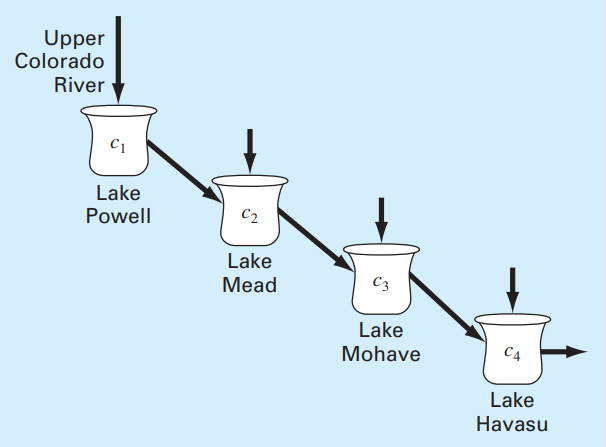
\includegraphics[width=0.75\textwidth]{fig_11_18}
	\caption{\textsf{The Lower Colorado River.}}
	\label{fig:fig_11_18}
\end{figure}


11.14 Polynomial interpolation consists of determining the
unique $(n - 1)$th-order polynomial that fits $n$ data points.
Such polynomials have the general form,
\begin{equation}
f(x) = p_{1}x^{n-1} + p_{2}x^{n-2} +···+ p_{n-1}x + p_{n}
\tag{P11.14}
\end{equation}
where the p's are constant coefficients. A straightforward
way for computing the coefficients is to generate n linear
algebraic equations that we can solve simultaneously for
the coefficients. Suppose that we want to determine the
coefficients of the fourth-order polynomial $f (x) = p_{1}x^{4} +
p_{2}x^{3} + p_{3}x^{2} + p_{4}x + p_{5}$ that passes through the following five
points: (200, 0.746), (250, 0.675), (300, 0.616), (400, 0.525),
and (500, 0.457). Each of these pairs can be substituted into
Eq. (P11.14) to yield a system of five equations with five
unknowns (the p's). Use this approach to solve for the coefficients. In addition, determine and interpret the condition
number


11.15 A chemical constituent flows between three reactors
as depicted in Fig. P11.15. Steady-state mass balances can
be written for a substance that reacts with first-order kinetics. For example, the mass balance for reactor 1 is
\begin{equation}
Q_{1,in}c_{1,in} - Q_{1,2}c_{1} - Q_{1,3}c_{1} + Q_{2,1}c_{2} - kV_{1}c_{1} = 0
\tag{P11.15}
\end{equation}
where $Q_{1,in}$ = the volumetric inflow to reactor 1 ($m^{3}/min$),
$c_{1,in}$ = the inflow concentration to reactor 1 ($g/m^{3}$), $Q_{i,j}$ = the flow from reactor i to reactor j ($m^{3}/min$), $c_{i}$ = the concentration of reactor i ($g/m^{3}$), k = a first-order decay rate (/min),
and $V_{i}$ = the volume of reactor i (m3). 

(a) Write the mass balances for reactors 2 and 3.

(b) If k = 0.1/min, write the mass balances for all three
reactors as a system of linear algebraic equations.

(c) Compute the LU decomposition for this system.

(d) Use the LU decomposition to compute the matrix inverse.

(e) Use the matrix inverse to answer the following questions: (i) What are the steady-state concentrations for
the three reactors? (ii) If the inflow concentration to the
second reactor is set to zero, what is the resulting
reduction in concentration of reactor 1? (iii) If the inflow concentration to reactor 1 is doubled, and the inflow concentration to reactor 2 is halved, what is the concentration of reactor 3?
\begin{figure}[H]
	\centering
	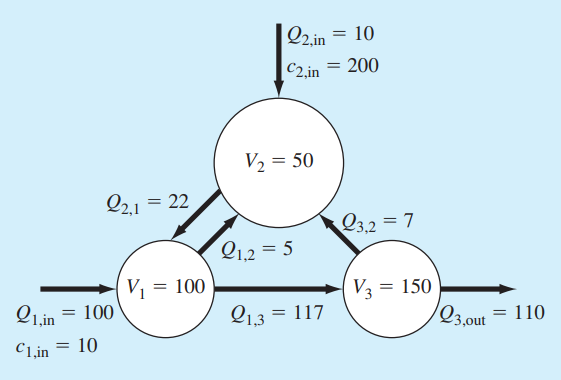
\includegraphics[width=0.75\textwidth]{fig_11_19}
	\label{fig:fig_11_19}
\end{figure}

\begin{figure}[H]
	\centering
	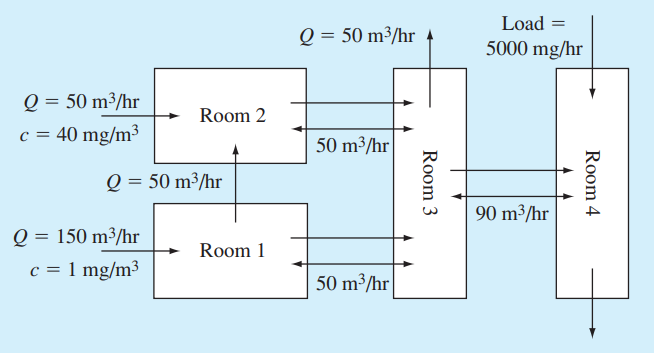
\includegraphics[width=0.75\textwidth]{fig_11_20}
	\label{fig:fig_11_20}
\end{figure}


11.16 As described in Examples 8.2 and 11.2, use the matrix
inverse to answer the following:

(a) Determine the change in position of the first jumper, if
the mass of the third jumper is increased to 100 kg.

(b) What force must be applied to the third jumper so that
the final position of the third jumper is 140 m?


11.17 Determine the matrix inverse for the electric circuit
formulated in Sec. 8.3. Use the inverse to determine the new
current between nodes 2 and 5 ($i_{52}$), if a voltage of 200 V is
applied at node 6 and the voltage at node 1 is halved.


11.18 (a) Using the same approach as described in Sec. 11.3,
develop steady-state mass balances for the room configuration depicted in Fig. P11.18.

(b) Determine the matrix inverse and use it to calculate the
resulting concentrations in the rooms.

(c) Use the matrix inverse to determine how much the room
4 load must be reduced to maintain a concentration of
20 $mg/m^{3}$ in room 2.

\end{document}

